\documentclass[a4paper]{article}


\usepackage[margin=2cm]{geometry}

\usepackage{graphicx,import}
\usepackage{color}
\usepackage{amsmath}
\usepackage{amssymb}

\usepackage{subcaption}

\usepackage{hyperref}
\usepackage{cleveref}

\newcommand{\bR}{\mathbb{R}}

\graphicspath{{figures/}}

\title{Separability of features learned with SGD}
\author{}

\begin{document}

\maketitle

\section{Goal, method}

The goal of this experiment is to evaluate the capacity of SGD of finding
classifiable features at different depths of an deep neural network first
trained end-to-end.

Input: $x \in \bR^d$ of dimension $d$, with $c$ classes.
\begin{itemize}
    \item
        First, a classifier is learned with a deep neural network ($L$ hidden
        layers). The training is performed until reaching $\varepsilon$ train
        error ($\varepsilon = 0$ for now)
    \item
        Then, $R$ is taken typically $R \ll \frac{n_L}{2}$. For each of the
        hidden layer $\ell$, $n_\ell -R$ features are randomly selected and fed
        into a new classifier of depth $L - \ell$, and of width equal to $R$.
    \item
        The training stops as soon as a random selection has led to $\varepsilon
        = 0$ training error on the dataset.
\end{itemize}

The cross-entropy loss is used for all the losses. SGD with momentum $\alpha =
0.95$ is used, with learning rate depending of the task.

\section{Network architectures}

\subsection{Original network}

$n_1, \ldots, n_L$: widths of the layers ($n_1 \geq n_2 \geq \cdots \geq n_L$).

Learning rate: $\lambda = 1e-3$.

\subsection{Feature classifier}

For each $\ell \in [L]$ depth of the original classifier, $n_\ell - R$ features
are selected uniformly at random (after the non-linear activation function has
been applied), and are fed into a $L - \ell$ deep network, with every layer of
width $R$. ReLU is also used, as well as cross entropy.

Learning rate: $\lambda = 1e-2$ for $L = 5$, $\lambda = 1e-3$ for $L = 10$.


\begin{figure}[!ht]
    \centering
    \begin{subfigure}{0.48\textwidth}
        \centering
    \import{drawing/}{original.pdf_tex}
    \caption{The original classifier deep network}
\end{subfigure}
    \begin{subfigure}{0.48\textwidth}
    \centering
    \import{drawing/}{classifier.pdf_tex}
    \caption{One of the subsequent classifier, of depth $L-\ell$.}
\end{subfigure}
\caption{The architecture of the networks}
\end{figure}


\section{Results}

\subsection{MNIST}

In this case, $c = 10, d = 748, n_1 = n_2 = \cdots = n_L = 500$.


SGD was able to produce classifiable features for depths $L = 5$ and $L = 10$,
removing respectively $R = 100$ and $R = 50$ neurons from an original $n = 500$
width (\cref{fig:mnist-classifier}).

It was possible to achieve $0$ training error with netowrks of depth $5$, width
$100$ and depth $10$, width $50$ (\cref{fig:mnist-small-width}).


\begin{figure}[!ht]
    \centering
    \begin{subfigure}{\textwidth}
        \centering
    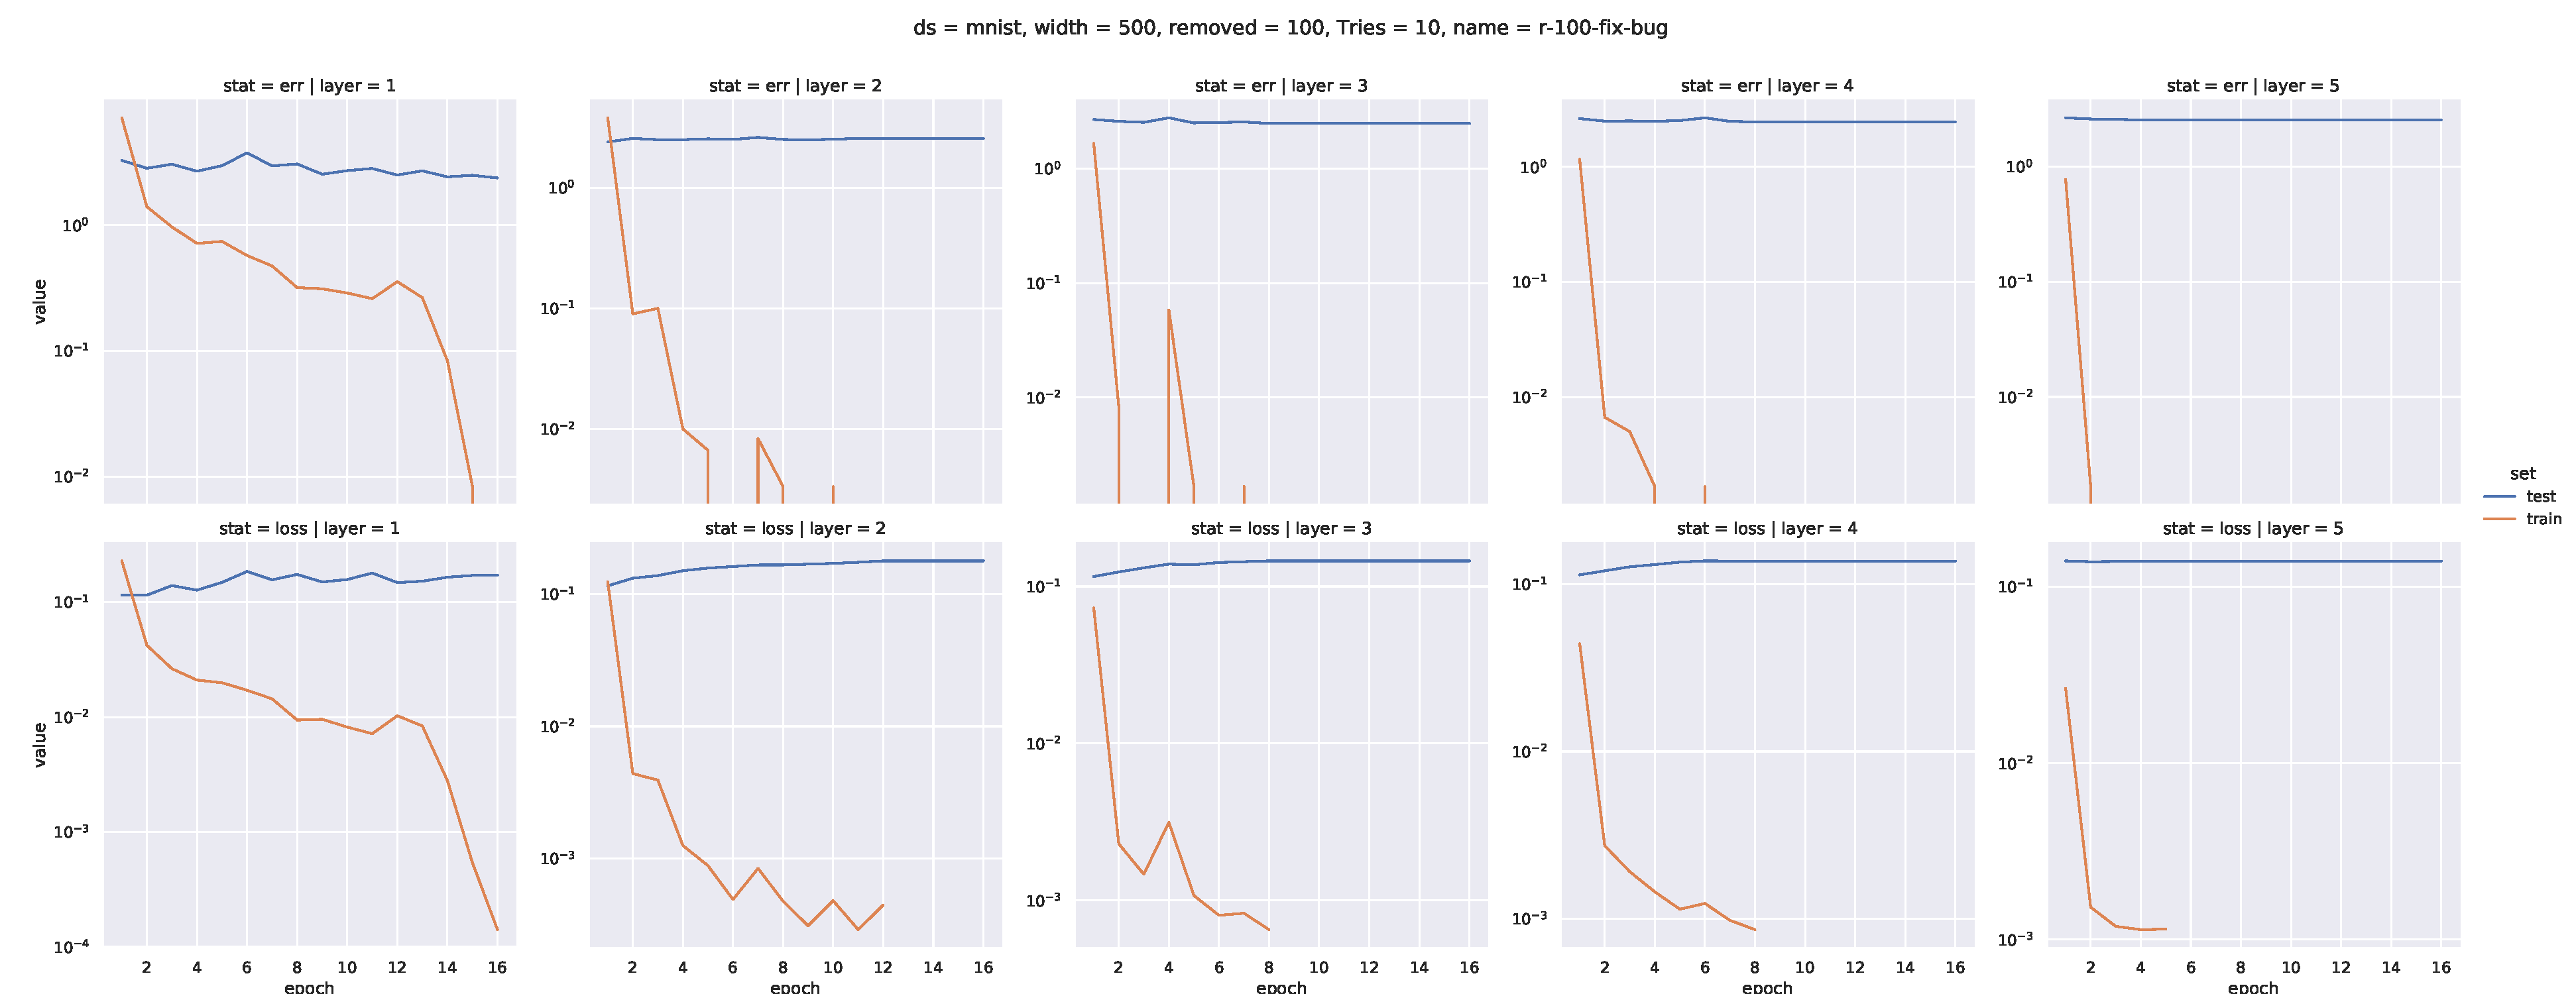
\includegraphics[width=\textwidth]{mnist/L_5_w_500_r_100}
\caption{$L = 5$, $R = 100$}
\end{subfigure}
\begin{subfigure}{\textwidth}
    \centering
    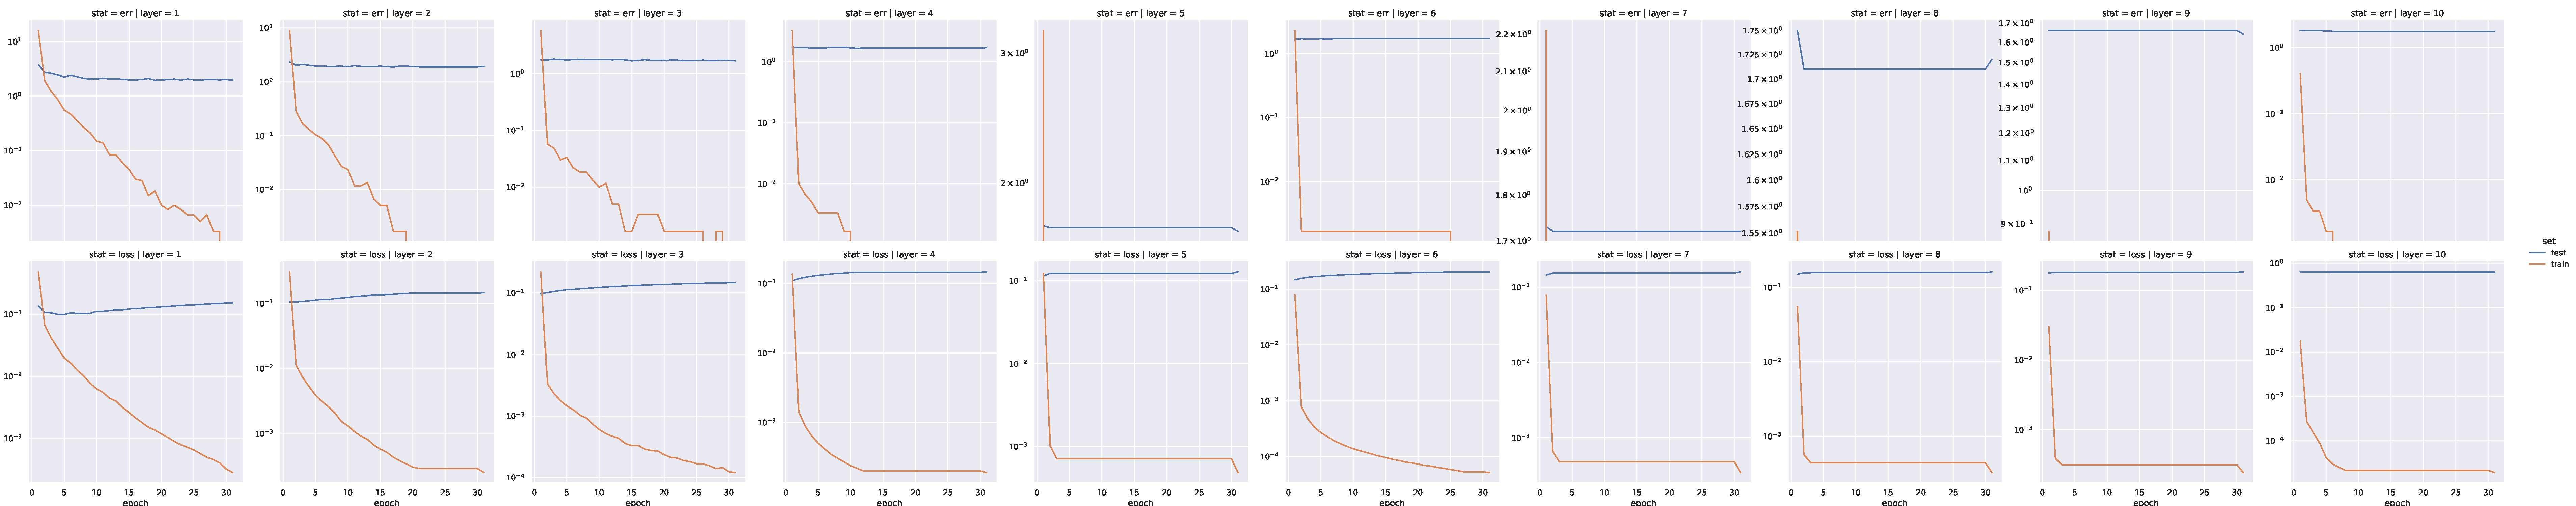
\includegraphics[width=\textwidth]{mnist/L_10_w_500_r_50}
    \caption{$L = 10$, $R = 50$}
\end{subfigure}
\caption{The different losses for the layers, $n_i = 500$, on MNIST.}
\label{fig:mnist-classifier}
\end{figure}

\begin{figure}[!ht]
    \centering
    \begin{subfigure}{0.24\textwidth}
    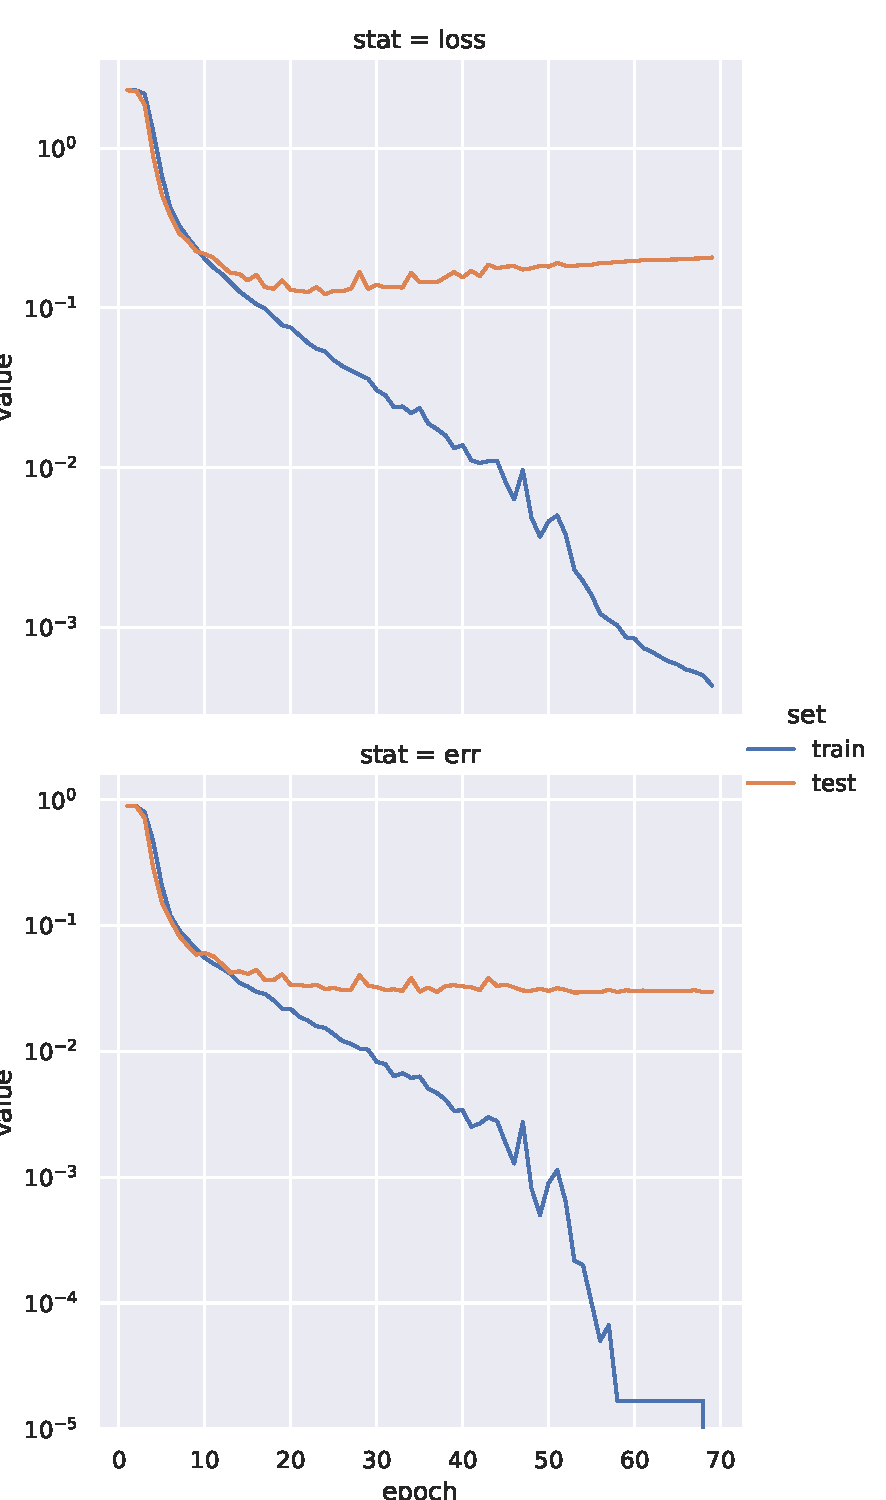
\includegraphics[width=\columnwidth]{mnist/L_5_w_100}
    \caption{$L = 5$, $n_i = 100$}
\end{subfigure}
\begin{subfigure}{0.24\textwidth}
    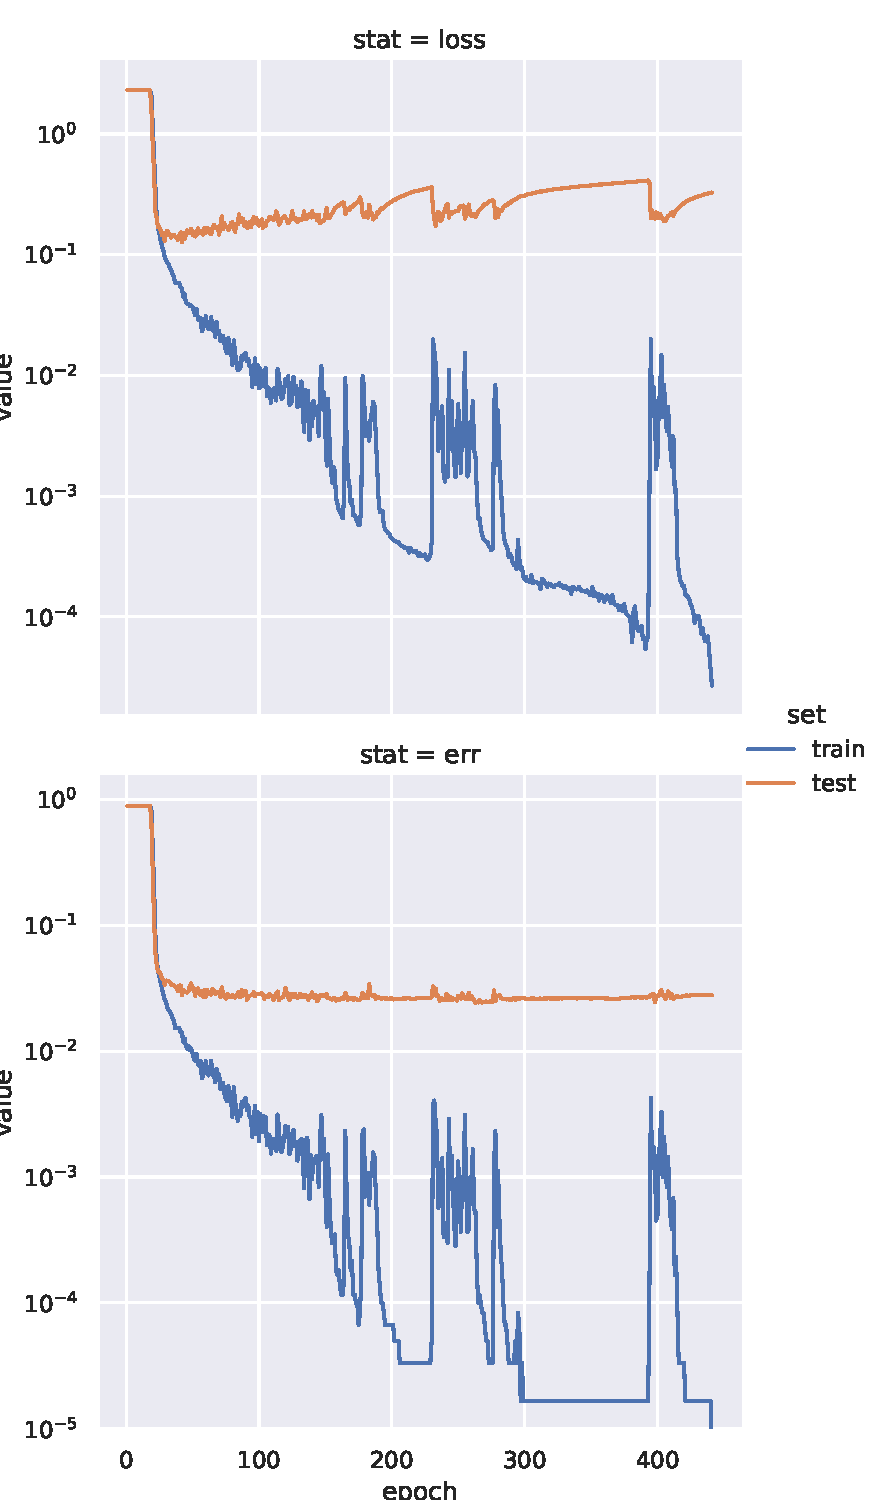
\includegraphics[width=\textwidth]{mnist/L_10_w_50}
\caption{$L = 10$, $n_i = 50$}
\end{subfigure}
\caption{Training a deep classifier end-to-end with small width on MNIST}
    \label{fig:mnist-small-width}
\end{figure}


\pagebreak

\subsection{CIFAR10}

With CIFAR10, separation was obtained with $L=5$, $R=100$ at all layers
(\cref{fig:cifar10-classifier-l5}) but fails for now on $L=10$, $R=50$
(\cref{fig:cifar10-classifier-l10}).

Note that here the first layer has width $n_1 = 2500$, while the others have
width $n_i = 500, i \geq 2$, since the input dimension is $d = 3072$.

Small width networks can classify the dataset (\cref{fig:cifar10-small-width}).

\begin{figure}[!ht]
    \centering
    \begin{subfigure}{\textwidth}
        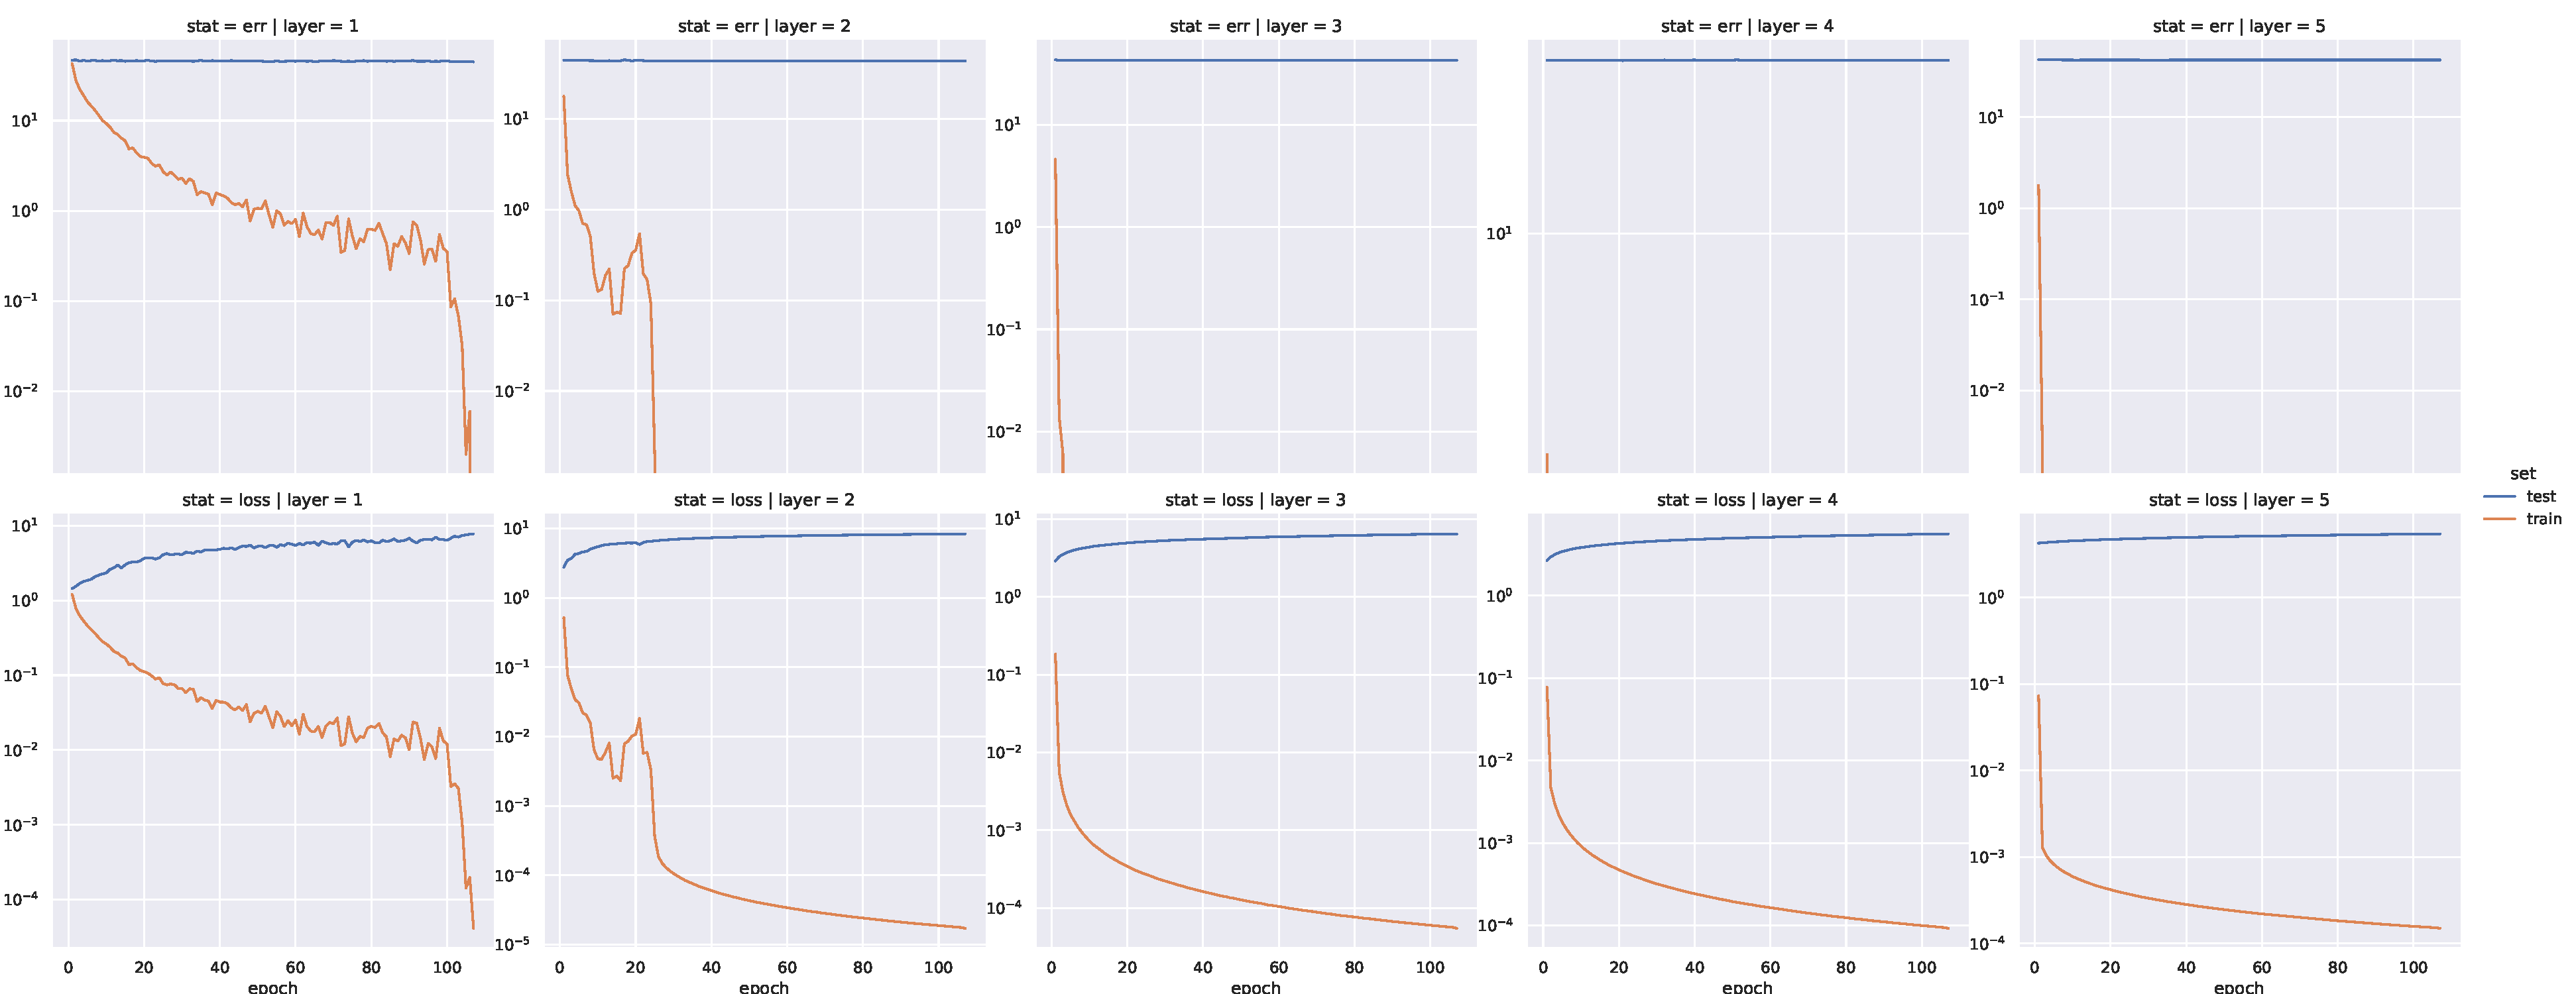
\includegraphics[width=\textwidth]{cifar10/L_5_n1_2500_w_500_r_100}
        \caption{$L = 5$, $R = 100$}
        \label{fig:cifar10-classifier-l5}
    \end{subfigure}
    \begin{subfigure}{\textwidth}
        \centering
    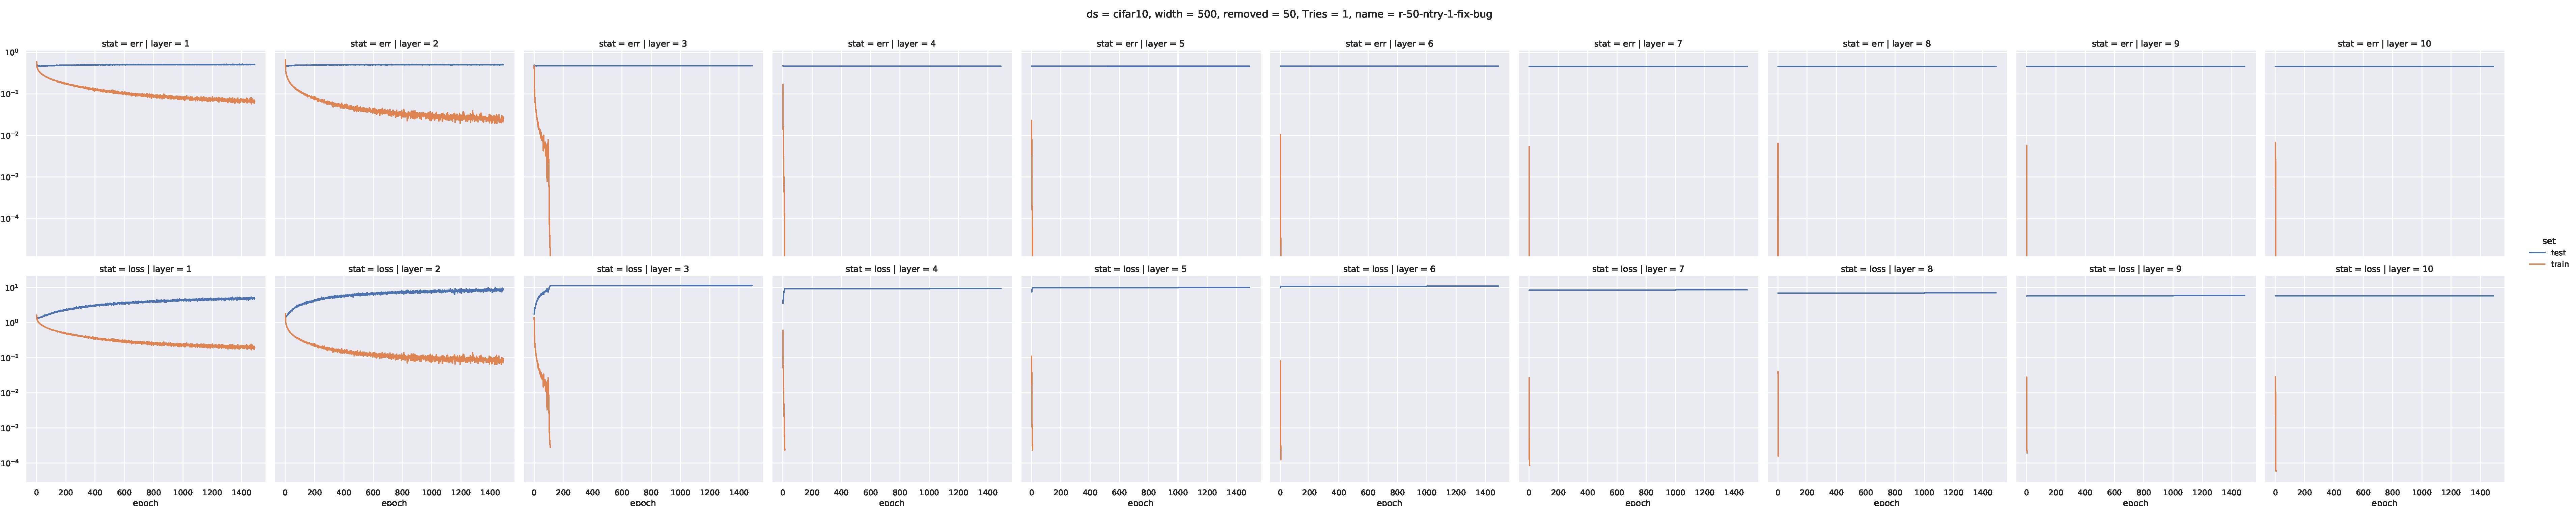
\includegraphics[width=\textwidth]{cifar10/L_10_n1_2500_w_500_r_50}
    \label{fig:cifar10-classifier-l10}
    \caption{$L = 10$, $R = 50$}
\end{subfigure}
\caption{The different losses for the modified classifier on CIFAR10, $d =
    3072$, $n_1 = 2500$, $n_{i \geq 2} = 500$. Each column $1 \leq \ell \leq L$ represents the
    loss of the classifier taking $n_\ell - R$ features of the layer $\ell$, and
    having depth $L-\ell$ }
    \label{fig:cifar10-classifier}
\end{figure}

\begin{figure}[!ht]
    \centering
    \begin{subfigure}{0.24\textwidth}
        \centering
    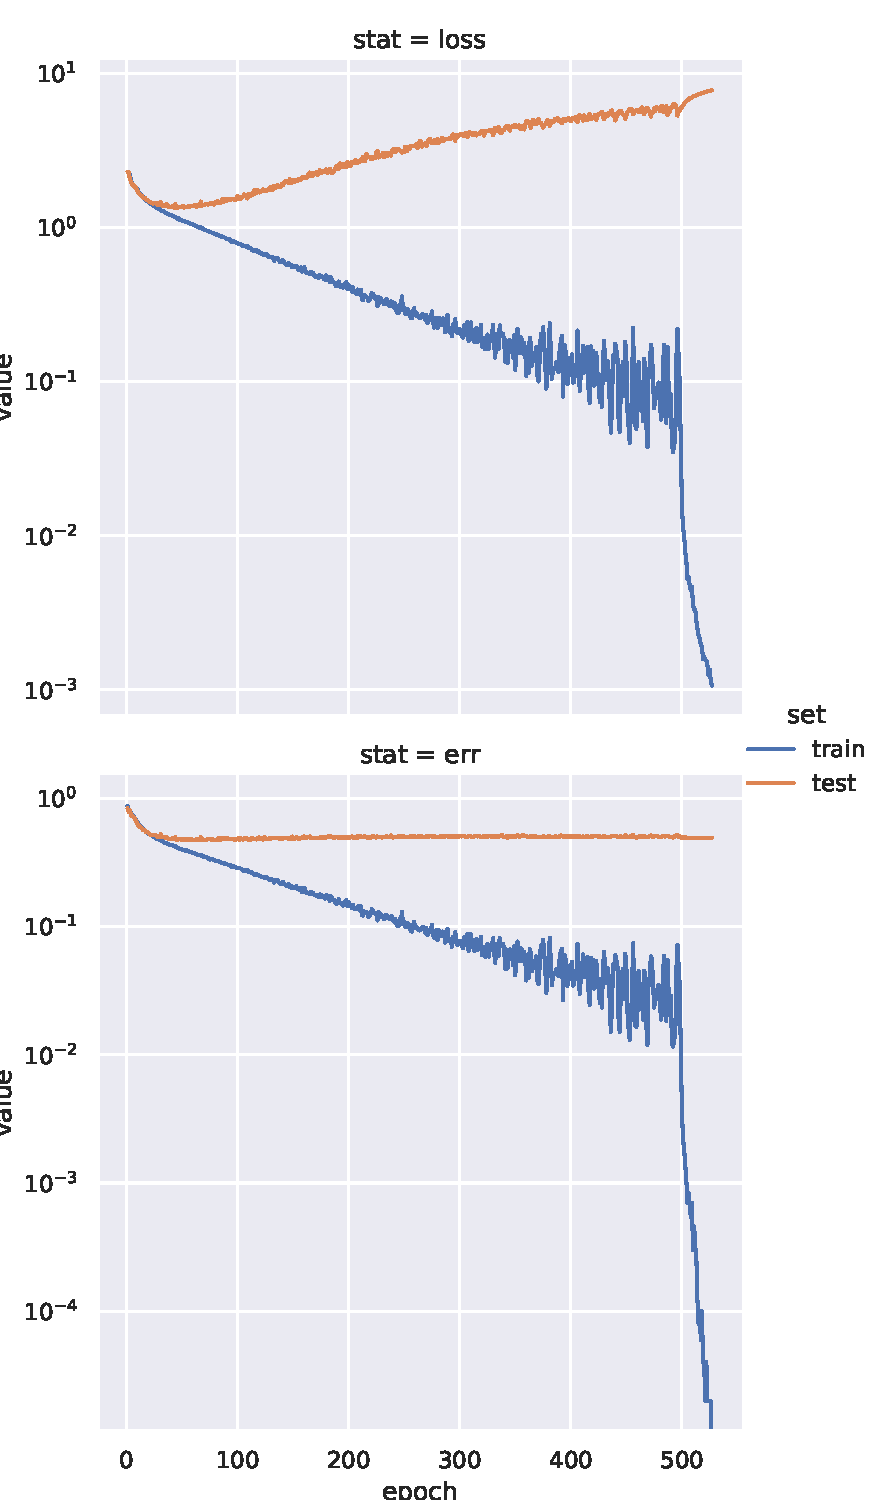
\includegraphics[width=\columnwidth]{cifar10/L_5_w_100}
    \caption{$L = 5$, $n = 500$}
\end{subfigure}
\begin{subfigure}{0.24\textwidth}
    \centering
    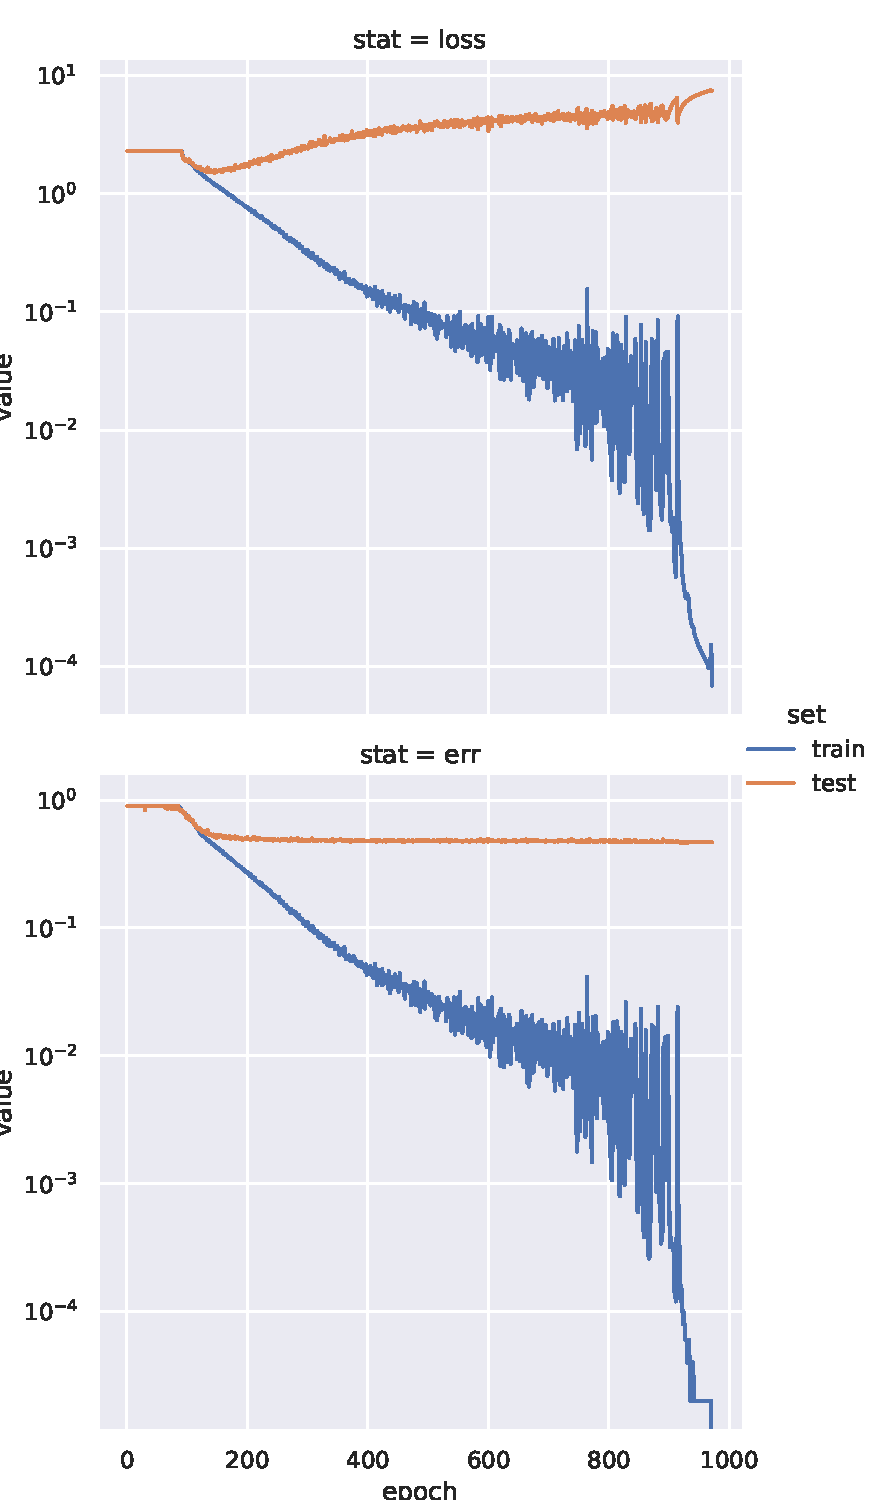
\includegraphics[width=\columnwidth]{cifar10/L_10_n1_2000_w_50}
    \caption{$L = 10$, $n_1=2000$, $n_i = 50$}
\end{subfigure}
\caption{Small width networks to classify CIFAR10}
\label{fig:cifar10-small-width}
\end{figure}








\end{document}
